
\section{Discussion and Research Gap}

% Chapter 4
% ======================================================================================================
% NOTES, TODOS
% limitation 
% Observation -> blockchain for data integrity and sharing Machine learning for intrusion detection cloud -> deploying dt in cloud 
% Privacy preserving 
% DT is a simulation platform 
% ======================================================================================================

In this literature review part of the project, we conducted a systematic way of reviewing the literature on the use of Digital Twin technology in Industry 4.0 domain to enhance security requirements. The study was carried out using the three-phase approach of conducting a systematic literature review that included designing a review protocol, conducting the review, and analysis. The aim was to investigate how Digital Twin is used to enhance security Industry 4.0. Besides, we explored the literature on what security scheme or mechanism is used to protect the integrity and confidentiality of data flow between (I)IoT devices and Digital Twin.


In this systematic literature review, we first performed a search on six electronic databases (ScienceDirect, SpringerLink, Scopus, IEEExplore, ACM, and Web of Science) yielded 727 papers. We then applied the inclusion and exclusion criteria listed in Table \ref{sec:inc-exc}, which resulted in 452 papers. Part of these criteria were already applied during the database search, such as the language, publication type, subject categories and publication year. Then we manually screen the titles, keywords, and abstracts of the 452 papers. This resulted in 83 papers that were eligible for full-text review. We then conducted a full-text review of the 83 papers and excluded 16 papers that were not relevant to our research question. The final set of 67 papers was included in our analysis.

% A total of 727 articles were identified from online digital databases, such as ScienceDirect, SpringerLink, Scopus, IEEExplore, ACM, and Web of Science. After applying inclusion and exclusion criteria and removing duplicates, we left with 67 research papers in which we perform analysis to answer our research questions.

We observed that publishing research studies on using Digital Twin as a security solution began in 2018, and the adoption of Digital Twin technology has been growing rapidly in various Industry 4.0 sectors leading to a significant surge in research articles over the past 6 years, particularly in years 2021 and 2022.

The contributions of the analysed literature varied from theoretical concepts to Digital Twin-based security platforms. However, the majority of the studies focused on providing a framework with theoretical concepts.


In the following section, first, we discuss the past, present and future status of Digital Twin. Then, we briefly look into how Digital Twin is used as a security tool. And finally, we reflect on security mechanisms discussed in the literature for protecting data flow between Digital Twin and (I)IoT.


\subsection{Observation and Findings}
As a result of a thorough review of the literature on the use of DT technology for securing (I)IoT applications and securing digital communication between DT and IoT devices, we have identified a few findings.


\subsubsection*{Past, Present, and Future of Digital Twin}
In its early days, the Digital Twin concept was used primarily as a model in the manufacturing industry. However, with the advent of enabling technologies such as (I)IoT, AI, and cloud computing, it has evolved into an integrated platform capable of providing a range of services beyond just modelling. Today, it is used in various industries to enhance the security of complex environments in addition to improving productivity and efficiency. In the future, digital twins are expected to incorporate even more technologies and integrate more deeply with humans through research on Human-Computer Interaction technology. 

\begin{figure}[H]
    \centering
    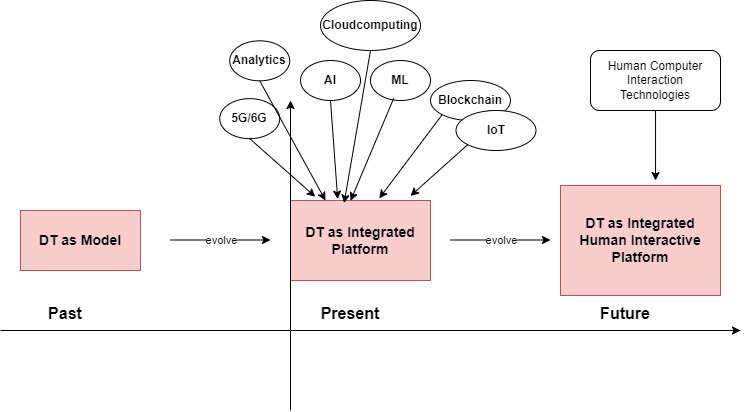
\includegraphics[width=\textwidth]{images/rt/dt-evolution.drawio.png}
    \caption{Evolution of Digital Twin Over Time}
    \label{fig:dt-evol}
\end{figure}


% \textbf{\textit{DT as integrated platform}}:
From the review, we identified Digital Twin as an integrated platform of a virtual model and enabling technologies to process collected data from the operating environment through (I)IoT sensors in order to gain insight for monitoring, optimization, and security purposes. 

One crucial aspect emphasized by authors for deploying a properly functioning Digital Twin is the necessity for real-time and uncorrupted data. A solution based on a lightweight and authenticated encryption algorithm might ensure that this requirement is met by ensuring that the data communicated between Digital Twin and the resource-constrained (I)IoT device is secured, meaning that the integrity of data is secured with authentication and the confidentiality of data with encryption.



\subsubsection*{Digital Twin as security tools}
Digital Twins have been developed for various purposes and use cases, including security. Our review indicated that it has mostly been used as a simulation platform for conducting testing and training. Next to using DT as a simulation, a number of solutions were proposed to detect anomalies \cite{chukkapalliCyberPhysicalSystemSecurity2021} and intrusions in cyber-physical systems(CPS) and industrial control systems (ICS) \cite{vargheseDigitalTwinbasedIntrusion2022, akbarianIntrusionDetectionDigital2020}. In this regard, the potential threats are DDoS, botnet activities, network breaches, and anomaly processes.   


The majority of papers discussed setting up a digital twin in a standalone environment to enhance the security of a targeted industry \cite{almeaibedDigitalTwinAnalysis2021, veledarDigitalTwinsDependability2019, chukkapalliCyberPhysicalSystemSecurity2021, adrienbacueDigitalTwinsEnhanced2022}. However, we found a few papers that presented the idea of sharing cyber threat intelligence(CTI) \cite{dietzHarnessingDigitalTwin2022, almeaibedDigitalTwinAnalysis2021} data generated using Digital Twin across industries to improve security collectively, which is a unique approach to using digital twin technology potentially having a significant impact on tackling big security problems, such as ransomware through sharable CTI. However, for this to be effective, we argue that the data-sharing process must happen in real-time with privacy in mind. 


In terms of enabling technologies, machine learning and data analytics are the core technologies used to power up Digital Twin to function as a security-enhancing tool. In other words, detection and protection security services are realized mainly using machine learning and data analytics that operate on extensive data collected through sensors. 


\subsection{Research Gap}
\label{sec:gap}
% \item\textbf{\textit{Lack of discussion on Lightweight encryption}}: 

In our review of selected papers, it became evident that most of the papers placed little emphasis on ensuring the authenticity and integrity of the sensor data that is fed into the Digital Twin. Even though a handful of papers discussed securing the data transmission channel, their recommendations relied on traditional encryption and authentication mechanisms such as AES, SHA-256 and RSA. 

This research gap and these proposals are concerning because in most use cases, the field sensors are power constraints where it is not feasible to deploy traditional encryption algorithms to secure them. Hence, it is important in future research to focus on lightweight algorithms to protect data confidentiality, integrity and authenticity of data used in Digital Twin-based solutions.



\subsection{Future Directions}

The application of Digital Twins for security in Industry 4.0 is at its early stage. While researchers have made significant contributions to its development, there are remaining research gaps that still require exploration and improvement. In this section, we identify and discuss three potential research area.

\textbf{\textit{Efficient lightweight encryption algorithms}}: As the development of Digital Twin technology progresses, it is expected that it will become accurate in replicating physical objects and processes. To achieve this level of accuracy, a large number of tiny, resource-constrained IoT sensors will need to be deployed on a massive scale to measure every aspect of the physical status being replicated. This presents future research directions for designing and implementing efficient encryption algorithms that can be deployed on resource-constrained devices.


% \textbf{\textit{Machine learning}}: Artificial intelligence(AI) is expected to play a crucial role in the future development of DT technology. Specifically, there are two potential areas where AI can be utilised: to perform analytics on collected data and to create AI-enabled simulations. Hence, future research could explore how machine learning technology is used in conjunction with DT models. This could involve conducting a systematic literature review to better understand how machine learning has been integrated within DT technology in previous research studies.

\textbf{\textit{Remote access control for DT}}: One area of research that we have identified as a gap in the literature is the secure remote access control to the virtual counterpart of an ICS component for vendors to perform troubleshooting and testing. In the traditional real-world industry setup, vendors of ICS components have remote access control to the physical object of the industry for various reasons. However, it is not clear how this is going to be handled on the DT yet. One potential direction for research is to explore and investigate how secure remote access can be achieved to one or more components of the DT.

% \textbf{\textit{DT based ransomware detection}}
\textbf{\textit{Human computer interaction}}: Finally, future research could explore the human-computer interaction (HCI) aspect of DT technology. This could involve examining how users interact with DT models and exploring new and innovative ways to improve the user experience. By improving the HCI aspect of DT technology, it may be possible to enhance the accuracy and reliability of the models by ensuring that human error is minimized.

\subsection{Limitations Of The Study}
% The concept of DT definition are not complete  
% Most study are focused on farmework 
% 
This study has two main categories of limitations: those related to collecting searching papers and those related to reviewing them.

\textbf{\textit{Limitations related to searching}}: Regarding the limitations related to collecting papers, the first issue is with the methodology used to select papers. Only papers with the exact phrase "[Dd]igital [Tt]win[s]?" in their title were collected for review. While the authors argue that research focused on digital twins will likely use this term in the title, this is not always the case. However, this approach also had the benefit of limiting the number of papers reviewed to those specifically discussing digital twins in security, instead of a potentially much larger set of papers. 

% Another limitation within this category is related to the three-stage searching mechanism employed to query papers from online archives. In one of the databases, we were unable to use the methodology directly as it lacked dedicated fields for searching the "abstract" sections of papers, unlike in the other libraries. However, we attempted to retrieve all papers with "digital twin*" in their title and at least one of the terms "security," "industry," or "IoT" and manually screened them to filter out the relevant ones.

\textbf{\textit{Limitation related to reviewing}}: There were multiple limitations associated with reviewing papers. First, most papers did not provide a complete and comprehensive definition of Digital Twin. Specifically, while the "state" component, encompassing both the virtual and physical states, was often explicitly described, the intended purpose and interconnectivity between these states were not consistently included in the definition.

 Another limitation within this category relates to the misunderstanding of Digital Twin as simulation software. Few papers, particularly within the healthcare sector, propose solutions utilizing simulation software under the consideration of Digital Twin. This view of Digital Twin as merely a simulation model or tool without bidirectional data flows between the Digital Twin and the mirrored real system may lead to confusion and potentially incorrect conclusions regarding the potential benefits and drawbacks of Digital Twin technology.

 Lastly, we observed that there needs to be more consistency in using the terms Framework, Methodology, and Architecture, which are often used interchangeably without a clear understanding of their definitions and distinctions. We argue that this could be due to a lack of consensus on how these terms should be used to categorize the contributions of authors. The inconsistency of the contribution categorisations in the analysed papers is particularly evident in cases where different terms are used to refer to the same things within a single paper, causing further ambiguity and hindering the accurate classification of the author's contributions.

 To address these limitations, reviewers had to carefully evaluate the definitions and concepts presented within papers by considering the broader context of the research to ensure a thorough understanding of the Digital Twin concept. In addition, it is crucial for researchers to establish clear definitions and appropriate usage of terms like framework, methodology, and architecture to facilitate effective communication and reliable classification of research contributions. By doing so, we have enhanced the quality and reliability of not only this research but might also enhance the quality and reliability of all future research related to Digital Twins.


\subsection{Conclusion of The Systematic Literature Review}
Overall, this systematic literature review based on 67 papers highlighted that Digital Twin technology is evolving to become vital technology, particularly in Industry 4.0. Industries such as the power grid, automotive industry, water treatment plants, transportation systems, smart cities, and satellite internet are a few of the sectors that benefited from Digital Twin. This technology offers real-time cybersecurity insights through an emulation environment for threat detection, vulnerability assessment, security awareness training, and threat intelligence. Luckily, these security measures can be implemented without disrupting the ongoing operations of these industries. 


% This systematic literature review, encompassing 69 papers, highlights the growing significance of Digital Twin (DT) technology in various smart industries. Industries such as the power grid, automotive sector, water treatment plants, transportation systems, smart cities, and satellite internet are recognizing the value of DT technology. It offers real-time cybersecurity insights by creating an emulation environment, enabling effective threat detection and response, vulnerability assessment, security awareness training, and threat intelligence. Importantly, these security measures can be implemented without disrupting the ongoing operations of these industries.

Based on the analysed papers, machine learning and data analytics are the two primary technologies that are widely used to enable digital twin security features. Due to the capability to analyse large amounts of data generated by Digital Twins, machine learning algorithms can be used to detect anomalies and identify potential security threats.

Digital Twin technology offers numerous benefits for Industry 4.0 use cases. But it also poses security challenges related to safeguarding the data collected and transmitted, especially with systems including storage, power and computationally constrained devices. Moreover, the SLR revealed that there is a limited amount of research on how to secure communication between DTs and resource-constrained devices. In other words, in most studies, security concerns related to the data used by Digital Twins during transmission were either neglected or traditional encryption methods are suggested. The most commonly suggested traditional encryption methods were AES, SHA-256 and RSA which are not feasible for deployment in devices with limited processing power and memory. This suggests that our hypothesis described in section \ref{sec:hypo} is correct. Hence, further study on designing and implementing lightweight cryptographic algorithms on these devices without compromising the desired level of security is required. 

We proposed using a lightweight encryption and authentication scheme to fill the research gap of unaddressed or inadequately addressed secure communication between resource-constrained (I)IoT devices and Digital Twin. In the following chapters, we present our proposed solution in addition to the implementation and validation of a proof of concept of this proposed solution in more detail. 

% To address the security-related issues of DT deployment, some researchers have proposed using blockchain technology to maintain the integrity and reliability of data when it is shared by a network of digital twins. Others suggested using tradition cryptographic mechanisms like RSA and AES to secure a data communication channel between the data source and the DT station hub. 

% Discussion on security
% XACML SAML and OAuth
% Quantum communication channel 
